\subsection{Hodge-Stern-Operator}
Der Hodge-Stern-Operator ist eine der drei Standard-Operationen auf dem Raum der Differentialformen. \\
Man spricht beim Kreuzprodukt von einer Rotation von Pseudovektoren, was nun anhand der Definition des Operators veranschaulicht werden soll. Wir werden sehen, dass die "Rechte-Hand-Regel" und die Metrik eingehen. \\
Ganz allgemein sei $V$ ein n-dimensionaler Vektorraum mit innerem Produkt $g$, induziert von der inversen Metrik, und ${\sigma^1, ..., \sigma^n}$ die geordnete Orthonormalbasis des Vektorraumes, sodass

\begin{align*}
g^{i j} := g(\sigma^{i},\sigma^{j}) = \pm \delta^{i j}.
\end{align*}


Der Hodge-Star-Operator ist abstrakt definiert als die Abbildung:
\begin{align*}
\star : \Lambda^p V \quad \rightarrow \quad  \Lambda^{n-p} V 
\end{align*}

mit der Eigenschaft

\begin{align}
\lambda \w \theta = (-1)^s g(\theta,\star\lambda) \omega
\end{align}

, wobei $\omega = \sigma^1 \w ... \w \sigma^n \in \Lambda^n V$, $\lambda \in \Lambda^p V$ und $\theta \in \Lambda^{n-p} V$. Dabei ist

 \begin{align}
 g(\omega,\omega) = \prod_{k=1}^{n} g(\sigma^{i},\sigma^{i}) = (-1)^s
 \end{align}
 
mit der Signatur $(s,n-s)$, wobei $s$ die Anzahl an $-$-Zeichen in der inversen Metrik ist.

 
Wir wollen mit einer etwas anschaulicheren, praktischeren Definition arbeiten, welche sich durch kleinere Umformungen aus der abstrakten Definition ergibt. \\

 Betrachten wir den Basis-p-Vektor $\lambda$ mit:
 \begin{align}
 \lambda = \sigma^1 \w \sigma^2 \w \dots \w \sigma^p = \sigma^{I} \quad \in \Lambda^p V
 \end{align}
 
 Einsetzen eines zweiten Basis-Vektors $\sigma^J \ \in \Lambda^{n-p}$ in die abstrakte Definition liefert:
\begin{align}
\lambda \w \sigma^J = (-1)^s g(\sigma^J,\star \lambda)\omega
\end{align}

Daraus folgt direkt $J = (p+1, ..., n)$ und 
\begin{align}
\star\lambda = \text{c} \cdot \sigma^{p+1} \w \dots \w \sigma^n.
\end{align}

Aus der Tatsache, dass $\lambda \w \sigma^J = \omega$ erhalten wir:

\begin{align}
1 = (-1)^s g(\sigma^J,\text{c}\cdot\sigma^J)
\end{align}

Oder Analog:
\begin{align}
\text{c}= \frac{(-1)^s}{g(\sigma^J,\sigma^J)} = \frac{g(\omega,\omega)}{g(\sigma^J,\sigma^J)} = g(\lambda,\lambda)
\end{align}

Alles zusammen führt zur der praktischen Definition des Operators als:
\begin{mybox}{Hodge-Stern-Operator}
\begin{align}
\star(\sigma^1 \w \sigma^2 \w \dots \w \sigma^p) = g(\sigma^1,\sigma^1)\dots g(\sigma^p,\sigma^p) \sigma^{p+1}\w \dots \w \sigma^n
\end{align}
\end{mybox}


 Für die zweifache Anwendung des Operators gilt: (ohne Herleitung)
 \begin{align}
 \star \star = \star^2 = (-1)^{p(n-p)+s}
 \end{align}






Eine alternative Definition des Operators, mit der wir ebenfalls noch arbeiten wollen, lautet (nun angewandt auf Differentialformen):
\begin{align}
\omega \w \star \mu = \left<\omega,\mu \right>\text{vol} = g(\omega,\mu)\alpha \quad \forall \omega, \mu \in \Omega^p(\mathcal{M}), \alpha \in \Omega^n(\mathcal{M})
\end{align}
Dabei ist $\text{vol} = \sqrt{\abs{\text{det} \ g_{\mu\nu}}} \ \dd x^1 \w \dots \w \dd x^n$ die Volumen-Form und $g_{\mu\nu}$ die Metrik. \\
\begin{figure}[H]
	\centering
	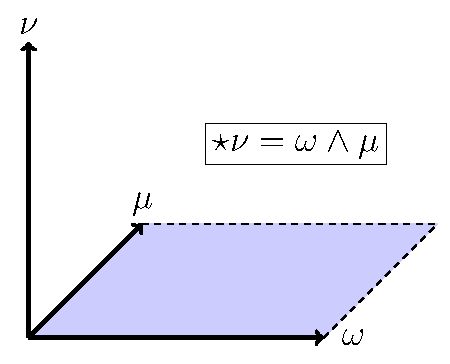
\includegraphics[width=.3\linewidth]{figures/darstellung-hodge.pdf}
	\caption{Grafische Darstellung der Funktion des Hodge-Stern-Operators}
\end{figure}
Beschränken wir den Operator auf den $\mathbb{R}^3$ verwenden wir nachfolgend die Notation $\star_s$.
\subsubsection{Anwendungsbeispiel: 4D-Minkowski-Raumzeit}

Wir betrachten den trivialen 4er-Vektor:

\begin{align}
\omega = - \dd t \w \dd x\w \dd y \w \dd z
\end{align}

Wenden wir nun den $\star$-Operator an, folgt zum Beispiel:

\begin{itemize}
\begin{align*}
\item \star 1 &= \omega \\
\item \star \omega &= -1 \\
\item  \star \dd t &= - \dd x \w \dd y \w \dd z \\
\item \star \dd x \w \dd y \w \dd z &= - \dd t \\
\item \star\star \omega &= (-1)^{4(4-4)+1} \omega = -\omega \\
\item \dots
\end{align*}
\end{itemize}

Wörtlich gesprochen liefert uns der Hodge-Stern-Operator die duale (n-p)-Form  zur p-Form durch "wedgen" der übrigen Basis-1-Formen, die nicht in der p-Form auftreten, unter Berücksichtigung der Geometrie des Raumes. \\
Dies wollen wir nutzen, um nun die inhomogenen Maxwell-Gleichungen neu auszuformulieren.

